\documentclass[border=10pt]{standalone}
\usepackage{tikz}
\usetikzlibrary{arrows.meta,positioning,calc,backgrounds}

\definecolor{ink}{HTML}{1F2933}
\definecolor{muted}{HTML}{7B8794}
\definecolor{arrowcol}{HTML}{4A5568}

\definecolor{laneAfill}{HTML}{F6F7F9}
\definecolor{laneAline}{HTML}{C3CAD3}
\definecolor{laneBfill}{HTML}{F4F8FD}
\definecolor{laneBline}{HTML}{B7C7DE}

\definecolor{amberfill}{HTML}{FDF2DC}
\definecolor{amberline}{HTML}{C4841D}
\definecolor{tealfill}{HTML}{E1F5F1}
\definecolor{tealline}{HTML}{12876F}
\definecolor{bluefill}{HTML}{E6EFFD}
\definecolor{blueline}{HTML}{2F6FED}
\definecolor{violetfill}{HTML}{EEE9FA}
\definecolor{violetline}{HTML}{6C4BD6}
\definecolor{greenfill}{HTML}{E5F6E9}
\definecolor{greenline}{HTML}{2E8B57}
\definecolor{rosefill}{HTML}{FCEBEF}
\definecolor{roseline}{HTML}{C2415F}

\renewcommand{\familydefault}{\sfdefault}

\newcommand{\nb}[2]{\textbf{#1}\\[1.5pt]{\scriptsize\color{muted}#2}}

\begin{document}
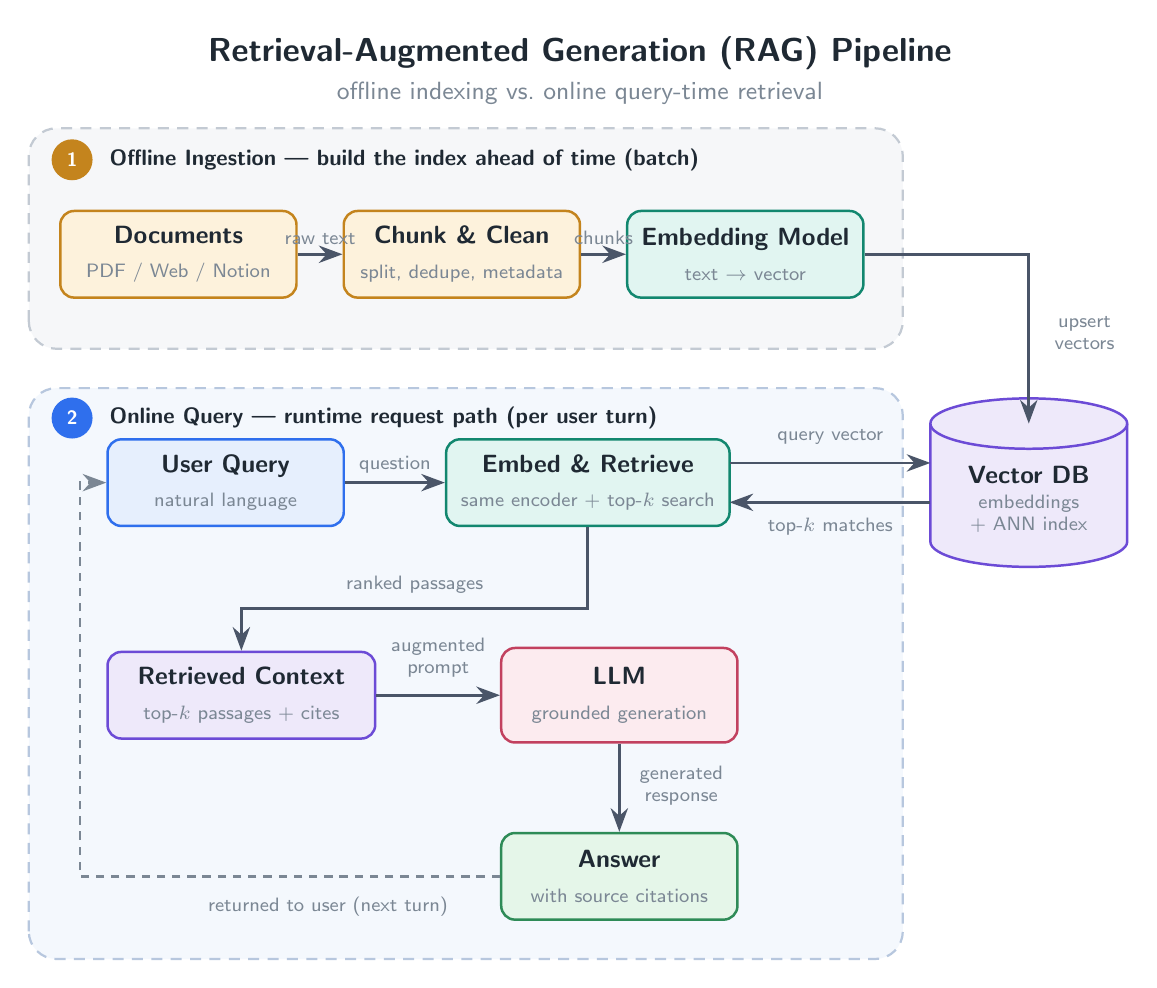
\begin{tikzpicture}[
  x=1cm, y=1cm,
  box/.style={
    draw, line width=0.9pt, rounded corners=5pt,
    minimum width=3cm, minimum height=1.1cm,
    align=center, inner sep=4pt, text=ink, font=\small
  },
  flow/.style={-{Stealth[length=3mm,width=2.2mm]}, line width=1pt, draw=arrowcol},
  back/.style={-{Stealth[length=3mm,width=2.2mm]}, line width=0.9pt, draw=muted, dashed, dash pattern=on 3pt off 2.5pt},
  lab/.style={font=\scriptsize, text=muted, align=center, inner sep=2pt},
  badge/.style={circle, draw=none, text=white, font=\bfseries\scriptsize, inner sep=0pt, minimum size=5.2mm}
]

%% ---------- title ----------
\node[font=\large\bfseries, text=ink] at (7.5,12.35) {Retrieval-Augmented Generation (RAG) Pipeline};
\node[font=\small, text=muted] at (7.5,11.85) {offline indexing vs.\ online query-time retrieval};

%% ---------- lanes ----------
\draw[rounded corners=10pt, line width=0.8pt, dashed, dash pattern=on 4pt off 3pt,
      draw=laneAline, fill=laneAfill] (0.5,8.60) rectangle (11.6,11.40);
\draw[rounded corners=10pt, line width=0.8pt, dashed, dash pattern=on 4pt off 3pt,
      draw=laneBline, fill=laneBfill] (0.5,0.85) rectangle (11.6,8.10);

\node[badge, fill=amberline] at (1.05,11.00) {1};
\node[lab, font=\footnotesize\bfseries, text=ink, anchor=west] at (1.45,11.00)
  {Offline Ingestion \textemdash\ build the index ahead of time (batch)};

\node[badge, fill=blueline] at (1.05,7.72) {2};
\node[lab, font=\footnotesize\bfseries, text=ink, anchor=west] at (1.45,7.72)
  {Online Query \textemdash\ runtime request path (per user turn)};

%% ---------- offline nodes ----------
\node[box, fill=amberfill, draw=amberline] (docs) at (2.4,9.80)
  {\nb{Documents}{PDF / Web / Notion}};
\node[box, fill=amberfill, draw=amberline] (chunk) at (6.0,9.80)
  {\nb{Chunk \& Clean}{split, dedupe, metadata}};
\node[box, fill=tealfill, draw=tealline] (emb) at (9.6,9.80)
  {\nb{Embedding Model}{text $\rightarrow$ vector}};

%% ---------- vector store ----------
\begin{scope}[shift={(13.2,6.90)}]
  \fill[violetfill]
    (-1.25,0.75) -- (-1.25,-0.75)
    arc[start angle=180, end angle=360, x radius=1.25, y radius=0.32]
    -- (1.25,0.75)
    arc[start angle=0, end angle=180, x radius=1.25, y radius=0.32] -- cycle;
  \draw[violetline, line width=0.9pt]
    (-1.25,0.75) -- (-1.25,-0.75)
    arc[start angle=180, end angle=360, x radius=1.25, y radius=0.32]
    -- (1.25,0.75);
  \draw[violetline, line width=0.9pt] (0,0.75) ellipse[x radius=1.25, y radius=0.32];
  \node[font=\small\bfseries, text=ink] at (0,0.10) {Vector DB};
  \node[font=\scriptsize, text=muted, align=center] at (0,-0.40) {embeddings\\+ ANN index};
\end{scope}
\coordinate (vdbN)  at (13.20,7.65);
\coordinate (vdbWa) at (11.95,7.15);
\coordinate (vdbWb) at (11.95,6.65);

%% ---------- online nodes ----------
\node[box, fill=bluefill, draw=blueline, minimum width=3cm] (uq) at (3.0,6.90)
  {\nb{User Query}{natural language}};
\node[box, fill=tealfill, draw=tealline, minimum width=3.6cm] (er) at (7.6,6.90)
  {\nb{Embed \& Retrieve}{same encoder + top-$k$ search}};
\node[box, fill=violetfill, draw=violetline, minimum width=3.4cm] (ctx) at (3.2,4.20)
  {\nb{Retrieved Context}{top-$k$ passages + cites}};
\node[box, fill=rosefill, draw=roseline, minimum width=3.0cm, minimum height=1.2cm] (llm) at (8.0,4.20)
  {\nb{LLM}{grounded generation}};
\node[box, fill=greenfill, draw=greenline, minimum width=3.0cm] (ans) at (8.0,1.90)
  {\nb{Answer}{with source citations}};

%% ---------- offline flow ----------
\draw[flow] (docs.east) -- (chunk.west)
  node[lab, midway, above=1pt] {raw text};
\draw[flow] (chunk.east) -- (emb.west)
  node[lab, midway, above=1pt] {chunks};
\draw[flow] (emb.east) -- (12.20,9.80) -- (13.20,9.80) -- (vdbN);
\node[lab, anchor=west] at (13.45,8.80) {upsert\\vectors};

%% ---------- online flow ----------
\draw[flow] (uq.east) -- (er.west)
  node[lab, midway, above=1pt] {question};

\draw[flow] (9.40,7.15) -- (vdbWa);
\node[lab] at (10.68,7.48) {query vector};
\draw[flow] (vdbWb) -- (9.40,6.65);
\node[lab] at (10.68,6.34) {top-$k$ matches};

\draw[flow] (er.south) -- (7.60,5.30) -- (3.20,5.30) -- (ctx.north);
\node[lab, anchor=south] at (5.40,5.42) {ranked passages};

\draw[flow] (ctx.east) -- (llm.west);
\node[lab] at (5.70,4.68) {augmented\\prompt};

\draw[flow] (llm.south) -- (ans.north);
\node[lab, anchor=west] at (8.18,3.05) {generated\\response};

\draw[back] (ans.west) -- (1.15,1.90) -- (1.15,6.90) -- (uq.west);
\node[lab, anchor=north] at (4.30,1.72) {returned to user (next turn)};

\end{tikzpicture}
\end{document}
